\documentclass[10pt]{article}
\usepackage[polish]{babel}
\usepackage[utf8]{inputenc}
\usepackage[T1]{fontenc}
\usepackage{amsmath}
\usepackage{amsfonts}
\usepackage{amssymb}
\usepackage[version=4]{mhchem}
\usepackage{stmaryrd}
\usepackage{graphicx}
\usepackage[export]{adjustbox}
\graphicspath{ {./images/} }

\title{KLASY PIERWSZE I DRUGIE }

\author{}
\date{}


\begin{document}
\maketitle
\begin{enumerate}
  \item Rozwiąż w liczbach naturalnych równanie
\end{enumerate}

\[
\frac{1}{x}+\frac{1}{y}+\frac{1}{z}=a
\]

\begin{enumerate}
  \setcounter{enumi}{1}
  \item Rozwiąż w liczbach całkowitych równanie
\end{enumerate}

\[
3 x^{2}+5 y^{2}=345
\]

\begin{enumerate}
  \setcounter{enumi}{2}
  \item Rozwiąż w liczbach pierwszych równanie
\end{enumerate}

\[
p q r=5(p+q+r)
\]

\section*{KLASY TRZECIE}
\begin{enumerate}
  \item Wyznacz wzór funkcji \(f(x)\), wiedząc, że \(f\left(\frac{2 x+3}{x-1}\right)=x+1\).
  \item Dany jest trójkąt \(A B C\). Niech \(D\) będzie punktem styczności okręgu wpisanego w ten trójkąt z bokiem AB, a E punktem styczności okręgu dopisanego do tego trójkąta z bokiem AB. Udowodnij, że |AD|=|EB|
  \item Niech \(p\) będzie dowolną liczbą pierwszą. Udowodnij, że\\
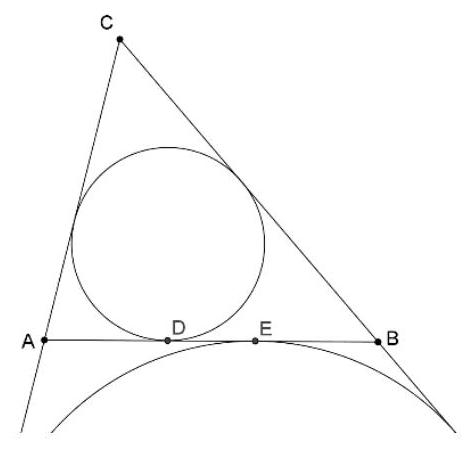
\includegraphics[max width=\textwidth, center]{2024_11_21_8a513b02f26bec178ccdg-1}\\
reszta z dzielenia liczby \(p\) przez 30 nie jest liczbą złożoną .
\end{enumerate}

\end{document}